\documentclass[aspectratio=169,14pt,usenames,dvipsnames]{beamer}
\usetheme{TalentSprint}
\usepackage[utf8]{inputenc}
\usepackage{graphics}
\usepackage{ragged2e}
\usepackage{amsfonts}
\usepackage{xcolor}
\usepackage{mathtools}
\usepackage{tcolorbox}
\usepackage{setspace}
\usepackage{lmodern}
\definecolor{swe}{rgb}{0.19, 0.73, 0.56}
\definecolor{lgreen}{RGB}{190,200,198}


\begin{document}

{\1
\begin{frame} \vspace{35pt}
	\title[ML Principles and  Practical Issues]{ML Principles and Practical Issues}
	\maketitle
\end{frame}
}

\begin{frame}[t]{The characteristics of good ML problems}
\centering
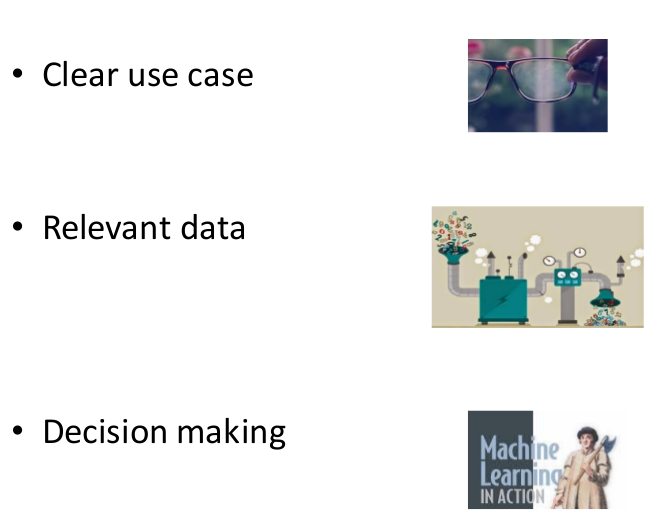
\includegraphics[width=0.9\textwidth, height=0.7\textheight]{Images/AIML_MLPrinciples_IMG1.png}
\end{frame}

\begin{frame}[t]{The ML Pipeline}
\centering
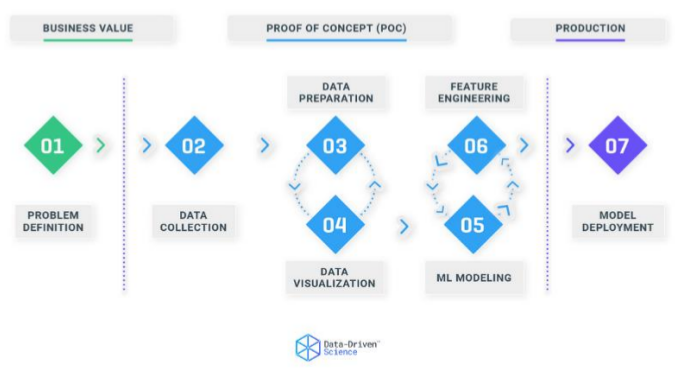
\includegraphics[width=0.8\textwidth, height=0.6\textheight]{Images/AIML_MLPrinciples_IMG2.png}\\
{\small{\url{https://medium.com/@datadrivenscience/7-stages-of-machine-learning-a-framework-33d39065e2c9}}}
\end{frame}

\begin{frame}[t]{A Hypothetical case study}
\begin{itemize}
  \item A lab scientist wants to build an automated system that will allow her cat in and out of her office window and disallow dogs from entering through it
\end{itemize}
\centering
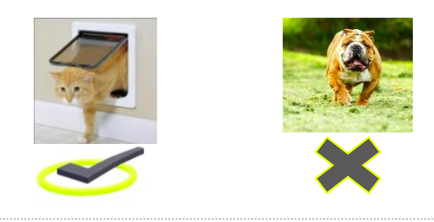
\includegraphics[width=0.7\textwidth, height=0.5\textheight]{Images/AIML_MLPrinciples_IMG3.png}
\end{frame}

\begin{frame}[t]{ML Problem formulation}
\begin{itemize}
\item ML Problem Statement: Classify cats vs dogs correctly
\end{itemize}
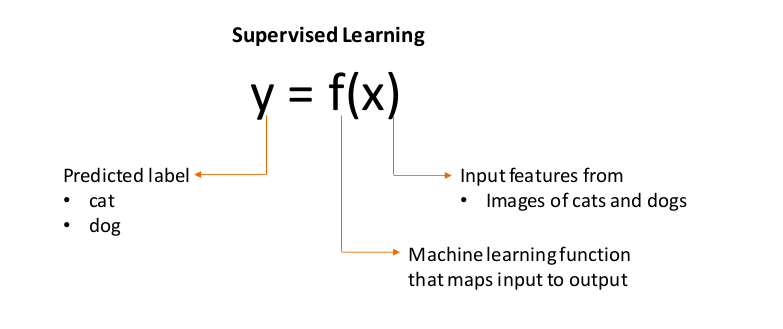
\includegraphics[width=0.9\textwidth, height=0.6\textheight]{Images/AIML_MLPrinciples_IMG13.png}
\end{frame}

\begin{frame}[t]{Build an ML classifier}
\centering
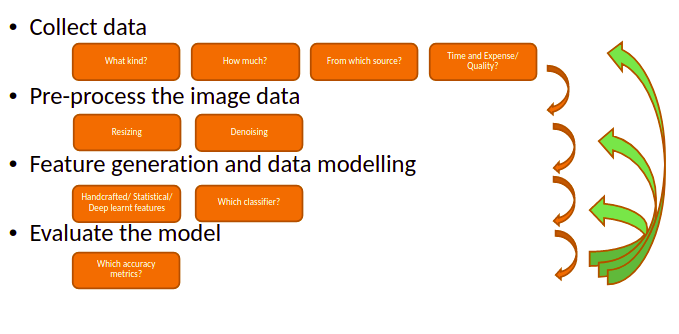
\includegraphics[width=0.9\textwidth, height=0.6\textheight]{Images/AIML_MLPrinciples_IMG4.png}
\end{frame}

\begin{frame}[t]{Practical issues}
\centering
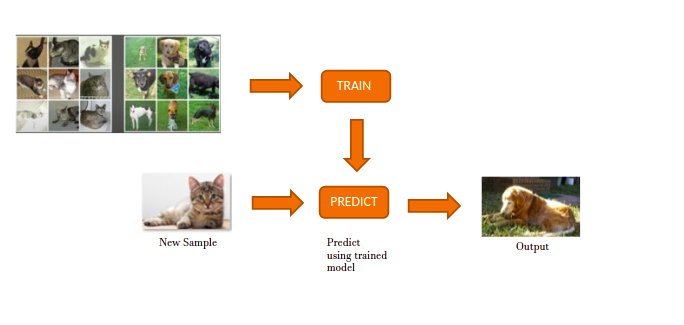
\includegraphics[width=0.9\textwidth, height=0.6\textheight]{Images/AIML_MLPrinciples_IMG5.png}
\end{frame}

\begin{frame}[t]{What could be the reasons?}
\centering
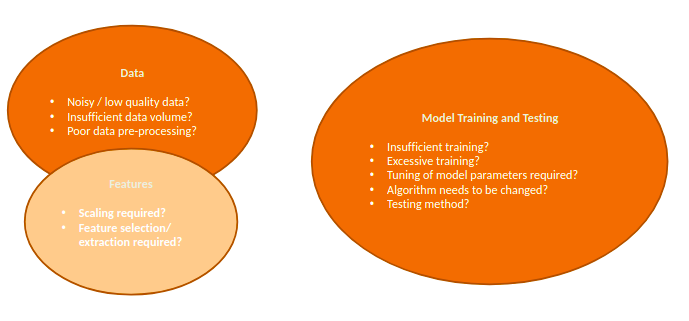
\includegraphics[width=0.7\textwidth, height=0.5\textheight]{Images/AIML_MLPrinciples_IMG6.png}
\end{frame}


\begin{frame}[t]{Holdout test set: The naive approach}
Randomly split the entire dataset into:
\begin{itemize}
\item \alert{Training set:} A dataset used for training the model	
\item \alert{Test set (a.k.a validation set):} Data only used for testing the model
\end{itemize}
\begin{center}
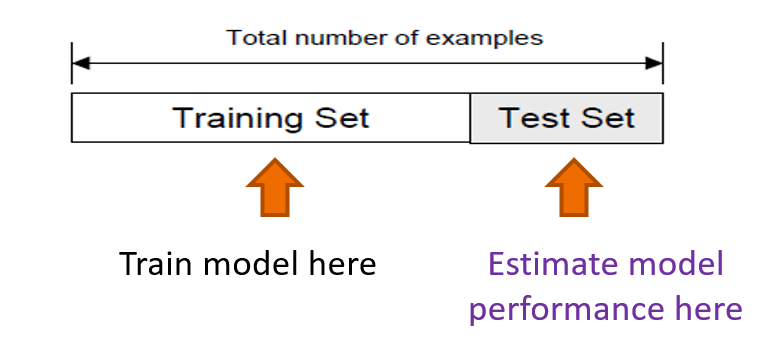
\includegraphics[width=7cm]{Images/AIML_MLPrinciples_IMG7.png}
\end{center}
\end{frame}


\begin{frame}[t]{The three-way split}
\begin{block}{Training set}
A set of examples used for learning
\end{block}
\begin{block}{Validation set}
A set of examples used to tune the parameters of a classifier
\end{block}
\begin{block}{Test set }
A set of examples used only to assess the performance of fully-trained classifier
\end{block}
\end{frame}


\begin{frame}[t]{The three-way split}
\begin{center}
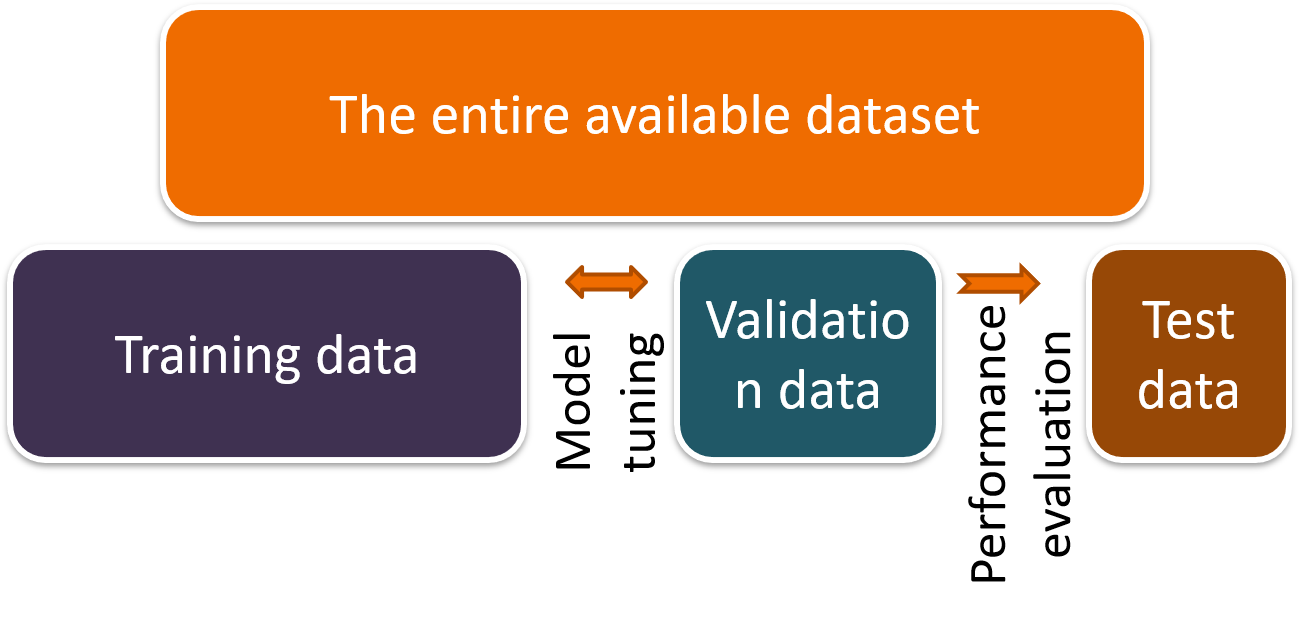
\includegraphics[width=11cm]{Images/AIML_MLPrinciples_IMG8.png}
\end{center}
\end{frame}


\begin{frame}[t]{How to perform the split?}
\begin{itemize}
\item How many examples in each data set? 
\begin{itemize}
\item \alert{Training:} Typically 60-80\% of data
\item \alert{Test set:} Typically 20-30\% of your data set
\item \alert{Validation set:}Around 20\% of data
\end{itemize}
\item Examples
\begin{itemize}
\item \alert{3 way:} Training: 60\%, Val: 20\%, Test: 20\%
\item \alert{2 ways:} Training 70\%, Test: 30\%
\end{itemize}
\end{itemize}
\end{frame}


\begin{frame}[t]{Holdout summary}
\begin{block}{Positive}
\begin{itemize}
\item Intuitive; Usually easy to perform; Considered the ideal method for evaluation
\end{itemize}
\end{block}
\begin{block}{Drawbacks:}
\begin{itemize}
\item In small datasets you do not have the luxury of setting aside a portion of your data
\item The performance will be misleading if we had unfortunate split
\end{itemize}
\end{block}
\end{frame}


\begin{frame}[t]{Common Splitting Strategies}
\begin{overlayarea}{14cm}{7cm}
\begin{itemize}
\uncover<3->{\item k-fold cross-validation}
\begin{center}
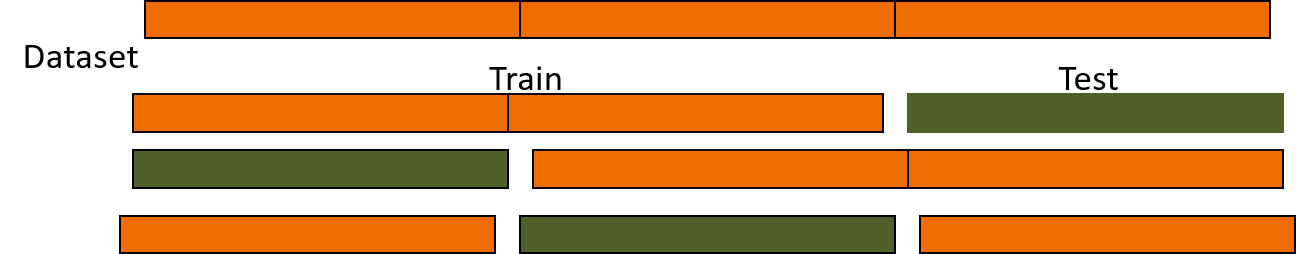
\includegraphics[width=11cm]{Images/AIML_MLPrinciples_IMG9.png}
\end{center}
\uncover<4->{\item Leave-one-out (n-fold cross validation)}
\begin{center}
\includegraphics<2->[width=11cm]{Images/AIML_MLPrinciples_IMG10.png}
\end{center}
\end{itemize}
\end{overlayarea}
\end{frame}


\begin{frame}[t]{Estimating model performance}
\centering
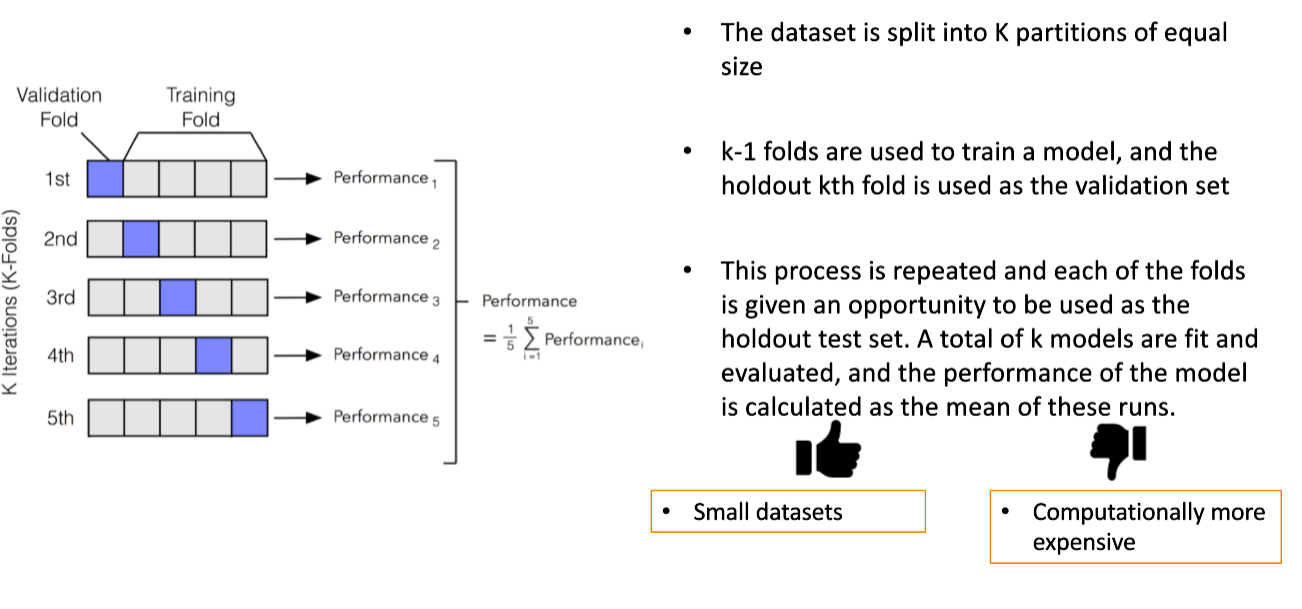
\includegraphics[width=0.7\textwidth, height=0.5\textheight]{Images/AIML_MLPrinciples_IMG11.png}
\end{frame}


\begin{frame}[t]{Cross - Validation}
\centering
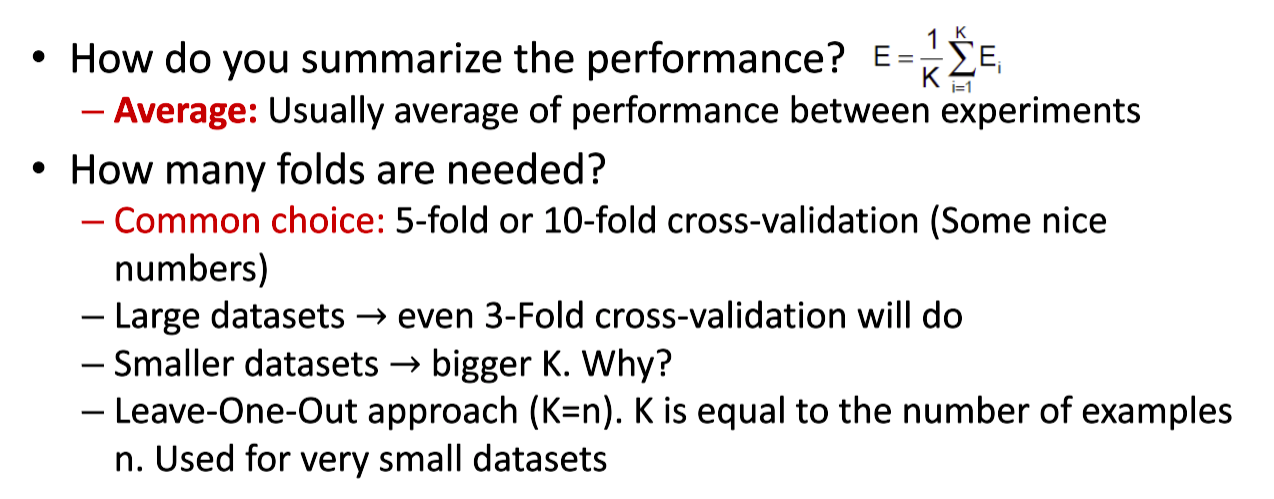
\includegraphics[width=0.9\textwidth, height=0.7\textheight]{Images/AIML_MLPrinciples_IMG12.png}
\end{frame}


{\1   
\begin{frame}
\title{Thanks!!}
	\subtitle{Questions?}
	\titlepage
\end{frame}
}

\end{document}
